\scanpage{534}
\mspage{570}
% E534-01
\[
\eta^{-1}\zeta={\varepsilon'_1}^{2\nu}\deleted{\unsure{=l_1^\nu}},
\quad\text{where }\nu=(\mu-1)/2,\quad\varepsilon'_1=-\varepsilon_1=\rho\sigma^{-1}
\]
% E534-02
we have
\[
{\varepsilon'_1}^{2\nu}=(-1)^{2\nu}\varepsilon_1^{2\nu}
=\varepsilon_1^{2\nu}=l_1^{\deleted{\unsure{2}}\nu},
\]
so the relation at the top takes the form
% E534-03
\[
\tag{16}
\boxed{\unsure{\zeta}=\eta l_1^\nu},\quad\text{where }\nu=(\mu-1)/2.
\]

% E534-04
We still have to prove the

\uline{Lemma} Let \unsure{$u$} be an \unsure{automorphism} of $\mathcal{G}$ such that $u(\sigma)$ is conjugate \inserted{in $\mathcal{G}$} to $\sigma$ or $\sigma^{-1}$, then
% E534-05
\[
\deleted{\unsure{u(-1)=-1|u(\sigma)^2=-1}}
\qquad\boxed{u(-1)=-1}
\tag{17}
\]
% E534-06
We will indeed have $u(\sigma)=\operatorname{int}(\alpha)(\sigma')$, \inserted{where $\sigma'=\sigma$ or $\sigma^{-1}$}, hence
\[
u(\sigma^2)=\operatorname{int}(\alpha)({\sigma'}^2)
=\operatorname{int}(\alpha)(-1)=-1,\quad\text{OK.}
\]

% E534-07
It remains \unsure{to|:} express \inserted{\unsure{finally}} that \deleted{$\zeta\rho$ is} $u(\rho)\inserted{=\operatorname{int}(\alpha)\rho}$ is conjugate to $\rho^\mu$, and $u(\sigma)$ to $\sigma^\mu$, and this is \deleted{\unsure{done by the conditions}} \inserted{\unsure{automatic}} for $\sigma$, since
% E534-08
\[
u(\sigma)=\operatorname{int}(\beta)\bigl(\varepsilon_2(\mu)\sigma\bigr)
=\operatorname{int}(\beta)(\sigma^\mu)\quad(\text{by }(9)),
\]
and for $\rho$ this means that we have
% E534-09
\[
\deleted{\unsure{\alpha\equiv\tau^{\varepsilon_3(\mu)}}}
\qquad\alpha\equiv\tau^{\nu_3(\mu)}\;(\mathcal{G})
\tag{17}
\]
\inserted{which we also write $\tau^{\nu_3(\mu)}\alpha\in\mathcal{G}$}
where $\nu_3(\mu)\inserted{\in\mathbb{Z}/2}$ is \unsure{the expression} additive \unsure{form|form} of $\varepsilon_3(\mu)$ —

% E534-10
So we have \unsure{found}

\uline{Corollary} \deleted{$B_{\rho,\sigma}$} The map
% E534-11
\[
\tag{18}
\diagram{\begin{tikzcd}[ampersand replacement=\&,column sep=large]
B_{\rho,\sigma} \arrow[r] \& \mathcal{G}\times\mathcal{G}\times\widehat{\mathbb{Z}}^{*} \\
(u,\mu) \arrow[r,mapsto] \& \bigl([u,\rho],[u,\sigma],\mu\bigr)
\end{tikzcd}}
\]
% E534-12
is injective, and it has as its image \unsure{the set}\inserted{$\Sigma_{\rho,\sigma}^{\mathrm{eff}}$} of triples $(\zeta,\eta,\mu)$ satisfying the following conditions:
% E534-13
\[
1^\circ)\quad\deleted{\text{the relation}}\quad
\zeta\rho\ \text{conjugate to }\inserted{\rho^\mu}\ \text{''}\ \rho^{\varepsilon_3(\mu)}\text{ in }\mathcal{G}
\]
% E534-14
\[
2^\circ)\quad\unsure{\eta|\zeta}\sigma\quad\rule{3.5cm}{0.3pt}\quad
\sigma^\mu=\sigma^{\varepsilon_2(\mu)}\text{ in }\mathcal{G}
\]
% E534-15
\margin{533}

% E534-F01
\margin{\begin{center}
533\\
\texttt{https://grothendieck.umontpellier.fr}\\
Université de Montpellier, UMR CNRS 5149, Case courrier 051, Place Eugène Bataillon\\
34095 Montpellier cedex 5 - France
\end{center}}

\scanpage{535}
% E535-01
3$^\circ$) We have the \uline{loop relation} (16).

% E535-02
4$^\circ$) $\exists$ automorphism $u$ of $\mathcal{G}$, satisfying
$u(\rho)=\zeta\rho$, $u(\sigma)=\eta\sigma$.

% E535-03
\deleted{For this, it \unsure{is necessary and sufficient} that we}

% E535-04
\unsure{The|The}
% E535-05
\inserted{conjunction of the}
conditions $1^\circ)$, $2^\circ)$, $3^\circ)$
\unsure{are equivalent|is equivalent} \unsure{to this}:
% E535-06
\deleted{\unsure{this one completes them}}
% E535-07
\inserted{this one:}

% E535-08
\[
\begin{gathered}
(A)\qquad
\exists(\alpha,\beta)\in\mathcal{G}'\times\mathcal{G},
\quad\text{with }\alpha\in\mathcal{G}\ \text{\unsure{sss|iff}}\ \mu\equiv1\ (3)
\\
\text{i.e. }\deleted{\unsure{\alpha}}\ 
\alpha\bmod\mathcal{G}=\tau^{\nu_3(\mu)},
\quad\text{and such that we have}
\\
\zeta=\alpha\rho(\alpha)^{-1},\qquad \eta=\varepsilon_2(\mu).
\end{gathered}
\]
% E535-09: deletion before alpha mod G is retained in E535-08.

% E535-10
Let us consider the homomorphism \unsure{of|of the} groups
% E535-11
\[
(19)\qquad
\diagram{\begin{tikzcd}[ampersand replacement=\&,column sep=large]
L_0 \arrow[r,"{\unsure{i_{L_0,B}}}"] \& B_{\rho,\sigma}\\
l \arrow[r,mapsto] \& (\operatorname{int}(l),1)
\end{tikzcd}}
\]

% E535-12
It is injective if we always assume
% E535-13
\[
(20)\qquad L_0\cap\uline{\unsure{\operatorname{Centr}}}(\mathcal{G})=\{1\},
\]
% E535-14
its image is \unsure{normal|invariant} for we have
% E535-15
\[
(21)\qquad
u\bigl(\unsure{i_{L_0,B}}(l)\bigr)
=i_{L_0,B}\bigl(u(l)\bigr)=i_{L_0,B}(l^\mu),
\]
% E535-16
where $\mu$ is the multiplier. We set
% E535-17
\[
(22)\qquad \gamma_{\rho,\sigma}=B_{\rho,\sigma}/\operatorname{Im}L_0,
\]
% E535-18
\deleted{We thus construct}
% E535-19
whence canonical exact sequence
% E535-20
\[
(23)\qquad
\diagram{\begin{tikzcd}[ampersand replacement=\&]
1\arrow[r]\&L_0\arrow[r]\&B_{\rho,\sigma}\arrow[r]\&
\gamma_{\rho,\sigma}\arrow[r]\&1
\end{tikzcd}}
\]
% E535-21
and we have a homomorphism (\unsure{deduced} from
% E535-22
$\diagram{\begin{tikzcd}[ampersand replacement=\&,column sep=small]
(u,\mu)\arrow[r,mapsto]\&\mu
\end{tikzcd}}$
by factoring through $\gamma_{\rho,\sigma}$)
% E535-23
\[
(24)\qquad
\diagram{\begin{tikzcd}[ampersand replacement=\&]
\gamma_{\rho,\sigma}\arrow[r,"{\unsure{\chi_\gamma}}"]\&
\widehat{\mathbb{Z}}^{*}
\end{tikzcd}}
\]
% E535-24
whose kernel is denoted $\gamma_{\rho,\sigma}^{+}$:
% E535-25
\deleted{\unsure{of}}
% E535-26
\[
(25)\qquad
\diagram{\begin{tikzcd}[ampersand replacement=\&]
1\arrow[r]\&\gamma_{\rho,\sigma}^{+}\arrow[r]\&
\gamma_{\rho,\sigma}\arrow[r]\&\widehat{\mathbb{Z}}^{*}\arrow[r]\&1
\end{tikzcd}}
\]
% E535-27
\margin{534}

% E535-F01
\margin{\begin{center}
534\\
\texttt{https://grothendieck.umontpellier.fr}\\
Université de Montpellier, UMR CNRS 5149, Case courrier 051, Place Eugène Bataillon\\
34095 Montpellier cedex 5 - France
\end{center}}

\scanpage{536}
% E536-01
\mspage{571}

% E536-02
\unsure{Let us consider|Let us study} the composite homomorphisms
% E536-03
\[
(26)\qquad
\diagram{\begin{tikzcd}[ampersand replacement=\&,column sep=large]
\gamma_{\rho,\sigma}\arrow[r,"{\chi_\gamma}"]\&
\widehat{\mathbb{Z}}^{*}\arrow[r,"{\varepsilon_2}"]\&\pm1\\
\gamma_{\rho,\sigma}\arrow[r,"{\chi_\gamma}"]\&
\widehat{\mathbb{Z}}^{*}\arrow[r,"{\varepsilon_3}"]\&\pm1
\end{tikzcd}}
\]
% E536-04
and let
% E536-05
\[
(27)\qquad
\left\{
\begin{aligned}
&\gamma'_{\rho,\sigma},\gamma''_{\rho,\sigma}
\subset\gamma_{\rho,\sigma}
\quad\text{subgroups of index }2,\\
&\hspace{12em}\text{defined by}\\
&\gamma'_{\rho,\sigma}=\operatorname{Ker}(\varepsilon_3\circ\chi_\gamma),
\quad
\gamma''_{\rho,\sigma}=\operatorname{Ker}\varepsilon_2\circ\chi_\gamma
\end{aligned}
\right.
\]

% E536-06
Now let
% E536-07
\[
(28)\qquad
G_{\rho,\sigma}
=\left(
\underbrace{B_{\rho,\sigma}\cdot\mathcal{G}}_{
\substack{(\frac12\text{ direct})\\ \simeq S_0G_{\rho,\sigma}}}
\right)/L_0,
\]
% E536-08
where
% E536-09
\[
(29)\qquad
\diagram{\begin{tikzcd}[ampersand replacement=\&,column sep=huge]
L_0\arrow[r,"{i_{L_0,B}}"]\&
\underbrace{\unsure{B_{\rho,\sigma}}\cdot\unsure{G_{\rho,\sigma}|\mathcal{G}}}\\
l\arrow[r,mapsto]\&\operatorname{int}(l)\cdot l^{-1},
\end{tikzcd}}
\]
% E536-10
whose image is \unsure{invariant}. We have a commutative diagram
% E536-11
\[
(30)\qquad
\diagram{\begin{tikzcd}[ampersand replacement=\&,column sep=small,row sep=small]
\&\mathcal{G}\arrow[dr]\&\\
L_0\arrow[ur,hook]\arrow[dr]\&\&G_{\rho,\sigma}\\
\&B_{\rho,\sigma}\arrow[ur,hook]\&
\end{tikzcd}}
\]
% E536-12
--- $\operatorname{Ker}(\mathcal{G}\longrightarrow G_{\rho,\sigma})
\simeq\operatorname{Ker}(L_0\longrightarrow B_{\rho,\sigma}]
\simeq L_0\cap\unsure{\operatorname{Centr}}(\mathcal{G})$
is trivial \unsure{according to|according to} (20),
which we are going to assume in what follows. We have a homomorphism of exact sequences
% E536-13
\deleted{introduced}
% E536-14
\[
(31)\qquad
\diagram{\begin{tikzcd}[ampersand replacement=\&,column sep=small,row sep=small]
1\arrow[r]\&L_0\arrow[r]\arrow[d,phantom,"\unsure{\cup}"]\&
B_{\rho,\sigma}\arrow[r,"{\delta_B}"]\arrow[d,hook]\&
\gamma_{\rho,\sigma}\arrow[r]\arrow[d,equal]\&1\\
1\arrow[r]\&\mathcal{G}\arrow[r]\&
G_{\rho,\sigma}\arrow[r,"{\delta_G}"]\arrow[dr,"{\chi_G}"']\&
\gamma_{\rho,\sigma}\arrow[d,"{\unsure{\chi_\gamma}}"']\&\\
\&\&\bigl[\&\widehat{\mathbb{Z}}^{*}\&\bigr]
\end{tikzcd}}
\]
% E536-15
\margin{535}

% E536-F01
\margin{\begin{center}
535\\
\texttt{https://grothendieck.umontpellier.fr}\\
Université de Montpellier, UMR CNRS 5149, Case courrier 051, Place Eugène Bataillon\\
34095 Montpellier cedex 5 - France
\end{center}}

\scanpage{537}
% E537-01
Let us set
% E537-02
\[
(32)\qquad
\left\{
\begin{aligned}
Z_\rho&=\operatorname{Centr}_{G_{\rho,\sigma}}(\unsure{\cdot}\rho)\\
Z_\sigma&=\operatorname{Centr}_{G_{\rho,\sigma}}(\sigma)
\end{aligned}
\right.
\]
% E537-03
\figure{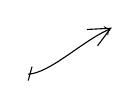
\begin{tikzpicture}[scale=.8]
\draw[->] (0,0) .. controls (.35,.02) and (.85,.52) .. (1.3,.72);
\draw (0,-.10)--(.06,.12);
\draw (.93,.71)--(1.31,.73)--(1.10,.45);
\end{tikzpicture}}

% E537-04
then the homomorphisms induced by $\delta_G$
% E537-05
\[
(33)\qquad
\diagram{\begin{tikzcd}[ampersand replacement=\&,column sep=large]
Z_\rho\arrow[r,"{\delta_\rho}"]\&\gamma_{\rho,\sigma}
\end{tikzcd}},
\qquad
\diagram{\begin{tikzcd}[ampersand replacement=\&,column sep=large]
Z_\sigma\arrow[r,"{\delta_\sigma}"]\&\gamma_{\rho,\sigma}
\end{tikzcd}}
\]
% E537-06
have
% E537-07
\deleted{as}
% E537-08
\inserted{some}
images which contain $\gamma'_{\rho,\sigma}$ and
$\gamma''_{\rho,\sigma}$ respectively,
% E537-09
\deleted{and \unsure{sss|iff} \unsure{to}}

% E537-10
\deleted{Moreover the image of $Z_\rho$ is contained in
$\gamma'_{\rho,\sigma}$
% E537-11
\deleted{if we assume}
% E537-12
\inserted{(\unsure{or equal}) \unsure{sss|iff}}
$\rho$ and $\rho^{-1}$ not conjugate in $\mathcal{G}$,
% E537-13
\deleted{it suffices}
% E537-14
\inserted{and}
% E537-15
\deleted{\unsure{for this}}
likewise the image of $Z_\sigma$ is
\unsure{reduced|reduced} to $\gamma''_{\rho,\sigma}$
\unsure{sss|iff} $\sigma$ and $\sigma^{-1}=-\sigma$
not conjugate in $\mathcal{G}$. Let us note for example
% E537-16
\deleted{that}
% E537-17
\inserted{if}
% E537-18
\deleted{$\mathcal{G}=\mathrm{SL}(2,\widehat{\mathbb{Z}})'$,}
$\sigma^2=1$,
\unsure{the} last condition is not \unsure{satisfied},
hence
% E537-19
$\diagram{\begin{tikzcd}[ampersand replacement=\&]
Z_\sigma\arrow[r]\&\gamma_{\rho,\sigma}
\end{tikzcd}}$
is surjective,
% E537-20
\deleted{it}
% E537-21
\inserted{\deleted{\unsure{but}} it}
is
% E537-22
\deleted{not either}
% E537-23
\deleted{\unsure{that it is satisfied if}}
$\mathcal{G}=\unsure{\mathrm{SL}}(2,\widehat{\mathbb{Z}})$
% E537-24
\inserted{in $\mathrm{SL}(2,\widehat{\mathbb{Z}})$}
$\sigma$ is conjugate there to $-\sigma$, by the
% E537-25
\deleted{(for $\sigma$ and}
general \unsure{theorem} of Steinberg for example) ---
\unsure{can it happen} in the universal \unsure{case}
$\mathrm{SL}(2,\mathbb{Z})^{\wedge}
=\mathcal{G}_{1,1}^{+\wedge}$?
}

% E537-26
\margin{\deleted{
The condition on $\rho$ is not satisfied
% E537-27
\deleted{\unsure{for}}
$\mathcal{G}=\mathrm{SL}(2,\widehat{\mathbb{Z}})/\pm1$,
As in this case the \uline{two} homomorphisms
% E537-28
$\diagram{\begin{tikzcd}[ampersand replacement=\&,column sep=small]
Z_\rho,\deleted{\unsure{Z_\sigma}}\arrow[r]\&
\unsure{\widehat{\gamma}_{\rho,\sigma}|\gamma_{\rho,\sigma}}
=\widehat{\mathbb{Z}}^{*}
\end{tikzcd}}$,
% E537-29
$\diagram{\begin{tikzcd}[ampersand replacement=\&,column sep=small]
Z_\sigma\arrow[r]\&\gamma_{\rho,\sigma}=\widehat{\mathbb{Z}}^{*}
\end{tikzcd}}$
are \unsure{surjections|surjective}),
but it is for $\mathcal{G}=\mathrm{SL}(2,\widehat{\mathbb{Z}})$,
for we find that the image of
% E537-30
$\diagram{\begin{tikzcd}[ampersand replacement=\&,column sep=small]
\unsure{Z_\rho}\arrow[r]\&\gamma_{\rho,\sigma}
\end{tikzcd}}$
is $\gamma'_{\rho,\sigma}$.
But in $\unsure{\mathcal{G}_{0,3}^{+\wedge}}$,
$\rho$ and $\rho^{-1}$ are also not conjugate,
i.e. the image is \unsure{reduced} also to $\gamma'_{\rho,\sigma}$.
}}
% E537-31
\margin{536}

% E537-F01
\margin{\begin{center}
536\\
\texttt{https://grothendieck.umontpellier.fr}\\
Université de Montpellier, UMR CNRS 5149, Case courrier 051, Place Eugène Bataillon\\
34095 Montpellier cedex 5 - France
\end{center}}